%% LaTeX-Beamer template for KIT design
%% by Erik Burger, Christian Hammer
%% title picture by Klaus Krogmann
%%
%% version 2.1
%%
%% mostly compatible to KIT corporate design v2.0
%% http://intranet.kit.edu/gestaltungsrichtlinien.php
%%
%% Problems, bugs and comments to
%% burger@kit.edu

\documentclass[18pt]{beamer}

%% SLIDE FORMAT

% use 'beamerthemekit' for standard 4:3 ratio
% for widescreen slides (16:9), use 'beamerthemekitwide'

\usepackage{templates/beamerthemekit}
% \usepackage{templates/beamerthemekitwide}

%% TITLE PICTURE

% if a custom picture is to be used on the title page, copy it into the 'logos'
% directory, in the line below, replace 'mypicture' with the 
% filename (without extension) and uncomment the following line
% (picture proportions: 63 : 20 for standard, 169 : 40 for wide
% *.eps format if you use latex+dvips+ps2pdf, 
% *.jpg/*.png/*.pdf if you use pdflatex)

%\titleimage{mypicture}

%% TITLE LOGO

% for a custom logo on the front page, copy your file into the 'logos'
% directory, insert the filename in the line below and uncomment it

%\titlelogo{mylogo}

% (*.eps format if you use latex+dvips+ps2pdf,
% *.jpg/*.png/*.pdf if you use pdflatex)

%% TikZ INTEGRATION

% use these packages for PCM symbols and UML classes
% \usepackage{templates/tikzkit}
% \usepackage{templates/tikzuml}

% the presentation starts here
\usepackage{graphicx}
\usepackage{listings}
\usepackage{color}
\usepackage{textcomp}
\definecolor{listinggray}{gray}{0.9}
\definecolor{lbcolor}{rgb}{0.9,0.9,0.9}
\lstset{
	language=Java,
	backgroundcolor=\color{lbcolor},
	tabsize=4,
	rulecolor=,
        basicstyle=\footnotesize,
        aboveskip=5pt,
        upquote=true,
        columns=fixed,
        showstringspaces=false,
        extendedchars=true,
        breaklines=true,
        frame=single,
        showtabs=false,
        showspaces=false,
        showstringspaces=false,
        identifierstyle=\ttfamily,
        keywordstyle=\color[rgb]{0,0,1},
        commentstyle=\color[rgb]{0.133,0.545,0.133},
        stringstyle=\color[rgb]{0.627,0.126,0.941},
}
\usepackage[utf8]{inputenc}

\title[Prog Tut Nr. 3]{Tutorium Programmieren}
\subtitle{Tut Nr.3: Checkstyle, Kontrollstrukturen}
\author{Michael Friedrich}
\date{12. / 14.11.2013}

\institute{Institut f\"ur theoretische Informatik}
% Bibliography

\usepackage[citestyle=authoryear,bibstyle=numeric,hyperref,backend=biber]{biblatex}
\addbibresource{templates/example.bib}
\bibhang1em

\begin{document}

% change the following line to "ngerman" for German style date and logos
\selectlanguage{ngerman}

%title page
\begin{frame}
	\titlepage
\end{frame}

%table of contents
\begin{frame}{Outline/Gliederung}
	\tableofcontents
\end{frame}

\section{Checkstyle}
\begin{frame}[fragile]{Checkstyle}
\begin{itemize}

	\item Beinhaltet Konventionen, um Code einheitlich und
	damit leserlich zu machen
	\begin{itemize}
	\item Wir bewegen uns im Spielraum, der uns der Compiler bietet
	\end{itemize}
	
	\item Daher Pflicht ab diesem Übungsblatt
	\begin{itemize}
	\item in 2 Stufen, vorerst nur Checkstyle 1
	\end{itemize}
	
	\item Daher Pflicht ab diesem Übungsblatt
	\begin{itemize}
	\item in 2 Stufen, vorerst nur Checkstyle 1
	\item Sonst: Abzug!
	\end{itemize}
	
\end{itemize}
\end{frame}

\begin{frame}[fragile]{Was beinhaltet Checkstyle?}
\begin{itemize}

	\item Zunächst, wie schon letzte Woche erwähnt
	\begin{itemize}
			\item Whitespace verpflichtend um
				\begin{itemize}
				\item = (Zuweisung)
				\item $+$, $+=$, $-$, $-=$
				\item \{, \}
				\item $==$, !$=$, $<, <=, >, >=$
				\item $\&\&, \mid\mid $
				\item if, else, for, while, return
				\item \ldots
				\end{itemize}
	\end{itemize}
\end{itemize}	
\end{frame}

\begin{frame}[fragile]{Was beinhaltet Checkstyle?}
\begin{itemize}

	\item Kein Whitespace nach
	\begin{itemize}
			\item Whitespace verpflichtend um
				\begin{itemize}
				\item $~$ (Bitweises Komplement)
				\item ++ (Prefix-Inkrementierung, z.B. ++i;)
				\item -- (Prefix-Dekrementierung, z.B. --i;)
				\item . (Punkt)
				\item - (Unäres Minus, z.B. -5)
				\item + (Unäres Plus, z.B. +4)
				\item \ldots
				\end{itemize}
	\end{itemize}
\end{itemize}	
\end{frame}


\begin{frame}[fragile]{Wie benutzt man Checkstyle?}
\begin{itemize}

	\item Kein Whitespace nach
	\begin{itemize}
			\item Whitespace verpflichtend um
				\begin{itemize}
				\item $~$ (Bitweises Komplement)
				\item ++ (Prefix-Inkrementierung, z.B. ++i;)
				\item -- (Prefix-Dekrementierung, z.B. --i;)
				\item . (Punkt)
				\item - (Unäres Minus, z.B. -5)
				\item + (Unäres Plus, z.B. +4)
				\item \ldots
				\end{itemize}
	\end{itemize}
\end{itemize}	
\end{frame}

\begin{frame}[fragile]{Wie benutzt man Checkstyle?}
\begin{itemize}

	\item Spätestens der Praktomat \textbf{prüft} ob ihr euch an die Richtlinien hält
	\begin{itemize}
			\item nur konforme Lösungen werden angenommen (ca. 3ÜB)
			\item Um einer stressigen Abgabe vorzubeugen, solltet ihr Checkstyle in eure IDE einbinden
			\item .xml Dateien auf \hyperlink{http://baldur.iti.uka.de/programmieren/}{http://baldur.iti.uka.de/programmieren/}
			
	\end{itemize}
\end{itemize}
\begin{center}
$\to$ Demo für Eclipse
\end{center}
\end{frame}

\section{Kontrollstrukturen}

\begin{frame}[fragile]{Kontrollstrukturen}
	\begin{block}{Wofür?}
	Kontrollstrukturen nutzen wir, um den linearen Programmfluss zu steuern.
		\begin{itemize}
			\item ermöglicht Fallunterscheidungen - \textbf{if}
			\item verhindert redundanten Code - \textbf{while}
		\end{itemize}
	\end{block}
\end{frame}

\begin{frame}[fragile]{Kontrollstrukturen}
\begin{exampleblock}{if-then-else - Verzweigungen}
	\begin{lstlisting}[basicstyle=\scriptsize]
				if (boolean1) {
							//code to run if boolean1 is true
				} elseif (boolean2) {
							//code to run if boolean2 is true AND boolean1 is false
				} else {
							//code to run otherwise
				}
	\end{lstlisting}
\end{exampleblock}
Hinweis: boolean kann auch ein zusammengesetzter Ausdruck sein
(Operatoren dazu siehe letztes Tut)
\end{frame}

\begin{frame}[fragile]{Kontrollstrukturen}
\begin{exampleblock}{while-Schleifen}
	\begin{lstlisting}[basicstyle=\scriptsize]
		while(boolean) {
			//code to run while boolean is true
		}
	\end{lstlisting}
\begin{center}
$\to$ Bedingung vor erstem Schleifendurchlauf erfüllt
\end{center}
\end{exampleblock}

\begin{exampleblock}{do-while - Schleifen}
	\begin{lstlisting}[basicstyle=\scriptsize]
		do{
			//code to run while boolean is true
		}while(boolean) 
	\end{lstlisting}
\begin{center}
$\to$ Was ist hier anders?
\end{center}
\end{exampleblock}
\end{frame}

\begin{frame}[fragile]{Kontrollstrukturen}
\begin{exampleblock}{for-Schleifen}
	\begin{lstlisting}[basicstyle=\scriptsize]
		for (var ; condition; var modification) {
			//code to run in loop
		}
	\end{lstlisting}
\end{exampleblock}

\begin{exampleblock}{Beispiel:}
	\begin{lstlisting}[basicstyle=\scriptsize]
		for (int i = 0; i < n; i++) {
		// loop
		}
	\end{lstlisting}
\begin{center}
Alternativ kann „i“ auch vorher initialisiert werden, die Zuweisung muss
aber hier geschehen. Vorteile?
\end{center}
\end{exampleblock}
\end{frame}


\begin{frame}[fragile]{Kontrollstrukturen}
\begin{exampleblock}{switch}
	\begin{lstlisting}[basicstyle=\scriptsize]
		switch (var) {
				case 1:
				// code if var is 1
				break;
				case 2:
				case 3:
				// code if var is 2 or 3
				break;
				default:
				// code to run if none of the above conditions hold
				break;
		}
	\end{lstlisting}
\end{exampleblock}
\begin{center}
Switch über \textbf{primitive Datentypen} möglich \newline
\small{Wie letztes Mal erwähnt ist String ein Sonderfall - Seit Java 1.7 auch (offiziell) möglich}
\end{center}
\end{frame}

\section{Getter / Setter}
\begin{frame}[fragile]{Getter / Setter}
\begin{itemize}
\item Methoden, die kontrollierten Zugriff auf Attribute ermöglichen, statt Zugriff mit Punkt
\end{itemize}
\begin{exampleblock}{Getter}
	\begin{lstlisting}[basicstyle=\scriptsize]
		returntype getVar(){
				return this.var;
		}
	\end{lstlisting}
\end{exampleblock}

\begin{exampleblock}{Setter}
	\begin{lstlisting}[basicstyle=\scriptsize]
		void setVar(varType param) {
			this.var = param;
		}
	\end{lstlisting}
\end{exampleblock}
\end{frame}

\begin{frame}[fragile]{Getter / Setter}
\begin{itemize}
\item Nutzen? 
\begin{itemize}
\item  Prinzip der \textbf{Kapselung}
\end{itemize}
\end{itemize}
 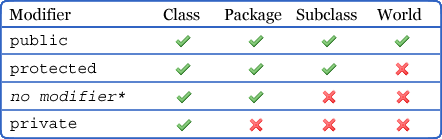
\includegraphics[width=1.0\textwidth]{pa.png}
\end{frame}

\section{Einschub}
\begin{frame}[fragile]{final und static}
\begin{itemize}
\item Es gibt 2 weitere Modifikatoren 
\end{itemize}
\begin{exampleblock}{final - definiert eine Konstante}
	\begin{lstlisting}[basicstyle=\scriptsize]
		final int MAX_VALUE;
	\end{lstlisting}
\end{exampleblock}
\begin{exampleblock}{static - definiert eine Klassenvariable}
	\begin{lstlisting}[basicstyle=\scriptsize]
		final static int NUMBER_OF_WHEELS;
	\end{lstlisting}
Klassenvariable bedeutet, dass dieses Attribut nicht an ein bestimmtes Objekt gebunden ist.
\end{exampleblock}
\end{frame}

\section{Tutoriumsaufgabe}
\begin{frame}[fragile]{Tutoriumsaufgabe}
\begin{itemize}
\item Wir wollen das bisher Gelernte umsetzen und uns einen eigenen Datentyp bauen \newline
			Die rationalen Zahlen
\end{itemize}
\begin{center}
	$\to$ Brainstorming
\end{center}
\end{frame}

\begin{frame}[fragile]{Tutoriumsaufgabe}
\begin{itemize}
\item Was brauchen wir also alles?
\begin{itemize}
	\item Ausgabe (toString)
	\item Addition
	\item Substraktion
	\item Beides mit int (Hinweis: Überladen)
	\item Kapselung
\end{itemize}
\end{itemize}
\end{frame}

\section{Ende}
\begin{frame}[fragile]{Das war's für heute}
\begin{center}
Danke für eure Aufmerksamkeit!\newline
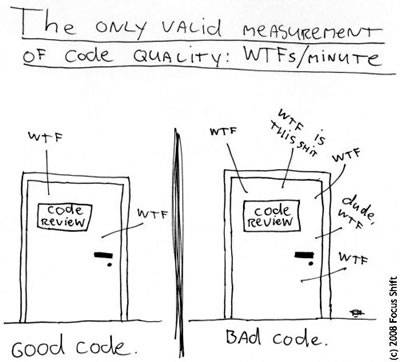
\includegraphics[width=0.6\textwidth]{wtf.png}
\end{center}
\end{frame}





\appendix
\beginbackup

%\begin{frame}[allowframebreaks]{References}
%	\printbibliography
%\end{frame}

\backupend

\end{document}
